\chapter{State of the Art}
\label{ch:state-of-the-art}

\section{The DNS System: Background}
\label{subsec:2.1}

The \ac{DNS} is the distributed directory that translates human-readable names into machine-readable information — primarily \ac{IP} addresses~\cite{RFC1034,RFC1035}. Its hierarchy mirrors the delegation of administrative authority: the root zone delegates to \ac{TLD}s, which delegate to authoritative name servers for individual domains. Resolution is performed by a recursive resolver acting on behalf of clients — contacting root, \ac{TLD}, and authoritative servers in sequence and caching results for the duration of each record’s \ac{TTL}.

Every \ac{RR} includes a \ac{TTL} that defines how long it remains in the cache. While \ac{CDN}s rely on short \ac{TTL}s (often 60 seconds or less) to dynamically reroute traffic, stable infrastructures typically set \ac{TTL}s of 24 hours or longer. This variance introduces critical challenges for active measurements. Relying on a recursive resolver risks retrieving outdated cached data. And different cache states across probes can easily be misinterpreted as geographic routing variations. Querying authoritative servers directly eliminates both of these confounding factors.

\subsection{Resource Record Types Relevant to Measurement Studies}
\label{sec:2.1.1}

\ac{DNS} stores information in typed Resource Records, each serving a distinct purpose \cite{RFC1035}. The record types most relevant to distributed measurement studies are:

\textbf{\ac{A} and \ac{AAAA} records} map a domain name to an \ac{IPv4} or \ac{IPv6} address respectively. A single name may have multiple \ac{A} or \ac{AAAA} records, enabling load distribution through round-robin responses and geographic routing through location-aware \ac{DNS} (different addresses returned depending on the querying resolver's location). This geographic differentiation in \ac{A}/\ac{AAAA} responses is one of the primary phenomena this thesis investigates.

\textbf{\ac{NS} records} designate the authoritative name servers responsible for a \ac{DNS} zone and are essential for identifying the \ac{DNS} infrastructure provider responsible for a domain. Van Rijswijk-Deij~\cite{vanRijswijk2016} include \ac{NS} records in the OpenINTEL standard query set because changes in \ac{NS} delegation reveal infrastructure migrations and provider switches.

\textbf{\ac{MX} records} designate the mail-handling servers for a domain. Van Rijswijk-Deij~\cite{vanRijswijk2016} use longitudinal \ac{MX} analysis as one of two case studies for OpenINTEL, tracking the adoption of cloud email services (Google Workspace, Microsoft Exchange Online, Yahoo Mail) across tens of millions of domains over a ten-month period.

\textbf{\ac{CNAME} records} create an alias pointing from one name to another canonical name. \ac{CDN}s make extensive use of \ac{CNAME} chains: a customer domain (\texttt{www.shop.example}) points to a \ac{CDN}-managed name (\texttt{shop.cdn-provider.net}), allowing the \ac{CDN} to update routing without requiring the customer to change their \ac{DNS} configuration. The same mechanism is used by \ac{DDoS} protection services to divert traffic through their scrubbing infrastructure~\cite{Jonker2016}.

\textbf{DNSKEY, DS, and RRSIG records} serve as the core cryptographic pillars of \ac{DNSSEC}, anchoring public keys, delegation signers, and digital signatures. To track \ac{DNSSEC} deployment and key management strategies on a global scale, Van Rijswijk-Deij~\cite{vanRijswijk2016} integrated this entire triad into the OpenINTEL query framework. By analyzing this specific longitudinal dataset, the authors were able to expose systemic key rollover failures that remained completely hidden during standard, point-in-time assessments.

\textbf{\ac{TXT} records} carry free-text information and are used for \ac{SPF}, \ac{DKIM}, \ac{DMARC} configuration, and domain validation tokens for certificate authorities. Table~\ref{tab:rr_types} summarises the record types relevant to this thesis's measurement campaign.

\begin{table}[H]
\centering
\small
\begin{tabularx}{\linewidth}{p{1.8cm} p{4.1cm} X}
\toprule
\textbf{Type} & \textbf{Content} & \textbf{Relevance for distributed \ac{DNS} measurement} \\
\midrule
\ac{A}     & \ac{IPv4} address(es)                  & Core observable: geographic variation in returned \ac{IP}s indicates \ac{CDN} routing or anycast \\
\ac{AAAA}  & \ac{IPv6} address(es)                  & Parallel to \ac{A}; anycast routing may differ between \ac{IPv4} and \ac{IPv6}~\cite{Bortzmeyer2013} \\
\ac{NS}    & Authoritative name server names   & Identifies \ac{DNS} provider; enables provider migration tracking and centralisation analysis~\cite{Xu2023} \\
\ac{CNAME} & Canonical name alias              & \ac{CDN} delegation chain; resolving the chain reveals the \ac{CDN} operator behind a domain \\
\ac{MX}    & Mail server hostname(s)           & Cloud email adoption tracking~\cite{vanRijswijk2016}; not geographically differentiated \\
\ac{TXT}   & Free-form text                    & \ac{SPF}/\ac{DKIM}/\ac{DMARC} policy; domain ownership verification \\
DNSKEY/DS & \ac{DNSSEC} public key / delegation & \ac{DNSSEC} deployment monitoring; broken chains cause SERVFAIL; 31\% of \ac{DNSSEC} domains have incomplete records~\cite{vanRijswijk2016,Chung2017} \\
\bottomrule
\end{tabularx}
\caption{\ac{DNS} \ac{RR} types relevant to distributed measurement studies. References: \cite{RFC1034,RFC1035}.}
\label{tab:rr_types}
\end{table}

\section{DNS Measurement Paradigms}
\label{sec:2.2}

Measuring \ac{DNS} behaviour at scale can be approached in fundamentally different ways, each with its own trade-offs in terms of coverage, geographic control, and ethical constraints. This section surveys the two main paradigms — passive and active measurement — along with the ethical framework that governs their use, and presents OpenINTEL as the reference large-scale active measurement infrastructure against which this thesis positions itself.

\textbf{Passive \ac{DNS}} captures queries and responses at existing resolvers or \ac{IXPs} without injecting artificial traffic. It reflects real user behaviour and is well suited for security forensics (botnet tracking, phishing detection via commercial services such as Farsight DNSDB). Its fundamental limitation for this thesis is geographic blindness: a passive sensor observes only traffic at its location~\cite{vanRijswijk2016}. It also cannot measure a predefined domain corpus, privacy constraints (GDPR) restrict retention granularity, and the resulting datasets are typically held by commercial operators (Farsight DNSDB, \ac{ISP}s), making them inaccessible for open academic research.

\textbf{Active \ac{DNS} measurement} deliberately sends queries from controlled vantage points, enabling full domain corpus coverage, geographic control, and reproducibility. Van Rijswijk-Deij~\cite{vanRijswijk2016} demonstrate that even at 1.85 billion daily queries for .com alone, well-paced active measurement represents only 0.3–1.6\% of authoritative server traffic — a negligible impact. Van der Toorn~\cite{vanderToorn2018} leverage 180 days of such data to detect snowshoe spam — a technique whereby spammers distribute sending across many domains to evade reputation-based blacklists — with 93\%+ precision and a 100-day lead over blacklists, a result exclusive to the active paradigm. Similarly, Jonker~\cite{Jonker2016} use 1.5 years of daily active measurements to track the adoption of \ac{DDoS} protection services across more than 50\% of the global namespace, revealing a 1.24$\times$ growth in adoption driven by large hosting providers — a trend invisible to any passive or point-in-time approach.

\textbf{Ethical framework}: As described by Kisteleki~\cite{Kisteleki2016}, RIPE Atlas measurement ethics align closely with the main principles of the Menlo Report (2012)~\cite{Bailey2012}, insisting that researchers must take full responsibility for the traffic generated by their probe hosts. In strict compliance with these principles, this thesis relies exclusively on publicly accessible Tranco domains. Furthermore, the experimental design intentionally avoids querying politically sensitive content and sets measurement frequency to respect standard \ac{DNS} \ac{TTL}s.

\textbf{OpenINTEL}~\cite{vanRijswijk2016}, developed at the University of Twente, measures every domain in a \ac{TLD} zone daily from a single vantage point in the Netherlands. It covers over 50\% of the global \ac{DNS} namespace, stores results in Apache Avro/Parquet, and has run continuously since March 2015. Its longitudinal data has supported studies of \ac{DNSSEC} key management failures~\cite{Chung2017}, \ac{DDoS} protection adoption~\cite{Jonker2016}, and cloud email migration~\cite{vanRijswijk2018blog}. Coverage expanded from the initial .com/.net/.org \ac{TLD}s (50\% of the global namespace) to all generic \ac{TLD}s by 2018, and the platform received the Research Data Netherlands Prize in November 2018~\cite{vanRijswijk2018blog}. Its explicit limitation is the single-vantage point architecture: whether a domain returns different \ac{IP} addresses to probes in Japan, Brazil, or South Africa is invisible to OpenINTEL — the primary motivation for the distributed approach of this thesis.


\section{Distributed Measurement: RIPE Atlas}
\label{sec:2.3}

Operated by a global network of volunteer-hosted hardware and software probes, RIPE Atlas offers the extensive spatial diversity that infrastructures like OpenINTEL lack. Data from 2024 shows the platform maintaining roughly 12,900 active probes (from a pool of over 30,000 registered devices) spanning 178 countries, which collectively yield around 1.3 billion daily measurement points~\cite{Nosyk2025}. Crucially, \ac{DNS} functionality is embedded as a native measurement type. Each probe perpetually tracks all 13 root server IP addresses, while custom user campaigns can be configured to target specific domains, resolvers, or record types. A detailed comparison between RIPE Atlas and alternative platforms is structured in Table~\ref{tab:platforms}.

\begin{table}[H]
\centering
\small
\begin{tabularx}{\linewidth}{p{2.6cm} r p{2.0cm} p{1.8cm} X}
\toprule
\textbf{Platform} & \textbf{Probes} & \textbf{Countries} & \textbf{\ac{DNS} native} & \textbf{Notes} \\
\midrule
RIPE Atlas       & $\approx$12,900 & 178 & Yes & Volunteer probes; credit economy; open academic access~\cite{Nosyk2025} \\
CAIDA Ark        & $\approx$170    & 60+ & No  & Topology-focused; data available on request to academic institutions; limited \ac{DNS} support~\cite{Bajpai2017} \\
SamKnows         & $\approx$70,000 & 50+ & No  & \ac{ISP}-deployed for regulators (FCC, Ofcom); not publicly accessible; broadband QoS focus~\cite{Bajpai2017} \\
PlanetLab        & $\approx$300    & 60+ & No  & Open to academic institutions (slice model); software VMs~\cite{Cicalese2015}; largely inactive since 2020 \\
BISmark          & $\approx$420    & 40+ & No  & Open source but limited access (Georgia Tech); home-network focus; limited geographic diversity~\cite{Bajpai2017} \\
\bottomrule
\end{tabularx}
\caption{Comparison of distributed Internet measurement platforms relevant to \ac{DNS} studies. Probe counts as of 2024 for RIPE Atlas~\cite{Nosyk2025} and approximately 2017 for others~\cite{Bajpai2017}. RIPE Atlas is the only platform with native \ac{DNS} measurement support and open academic access at global scale.}
\label{tab:platforms}
\end{table}

\textbf{Probe selection}: Bajpai~\cite{Bajpai2017} distinguish system tags (automatically derived from RIPE Atlas built-in measurements every four hours, reliable) from user tags (manually set by probe hosts; only 2.8\% ever update them, making them frequently stale). The recommended selection protocol is: filter by system tags (system-ipv4-works, system-resolves-a-correctly), then stratify geographically to compensate for the 91\% Europe/North America concentration. Holterbach~\cite{Holterbach2015} further document measurement interference: concurrent campaigns on the same probes introduce timing errors of 1–7 ms and temporal de-synchronisation of up to one hour. Scheduling at off-peak times and using repeated measurements mitigate both effects.

\textbf{Geographic bias}: A significant concentration of infrastructure exists in Germany and the USA, which combined host 28\% of all active probes. Conversely, regions such as Africa, Latin America, and Southeast Asia remain severely under-represented when compared to their actual Internet user populations~\cite{Nosyk2025}. This uneven global footprint is illustrated in Figure~\ref{fig:ripe_atlas_distribution}. Consequently, implementing strict geographic stratification during the probe selection phase becomes essential to accurately capture worldwide \ac{DNS} variations.

\begin{figure}[tp]
  \centering
  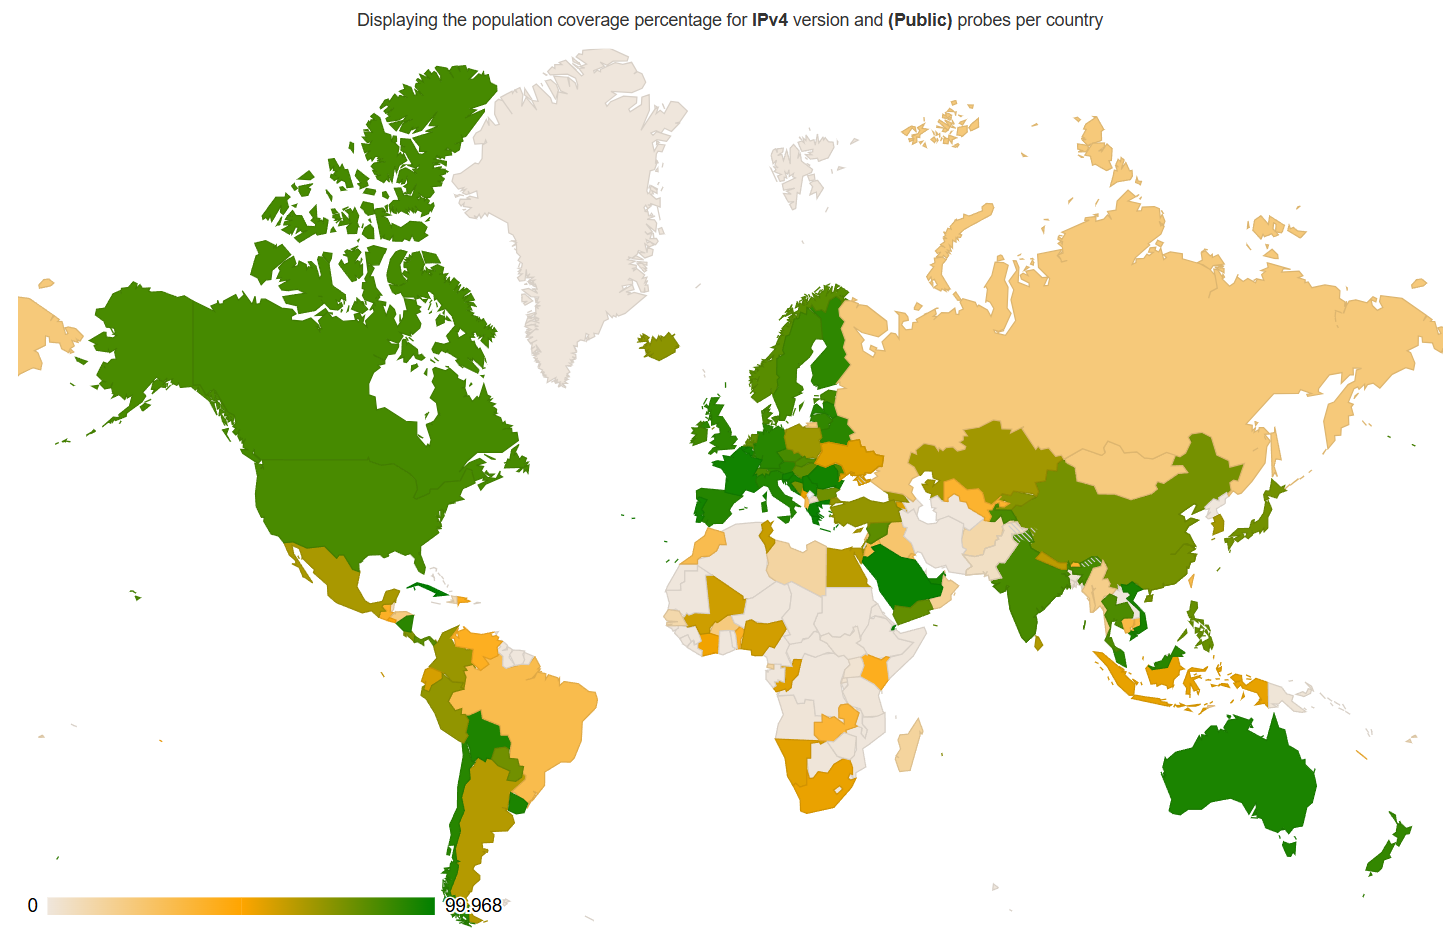
\includegraphics[width=0.90\linewidth]{figures/fig3b_ripe_atlas_distribution.png}
  \caption{Number of connected RIPE Atlas probes and anchors per country in March 30, 2026. Source: RIPE Atlas}
  \label{fig:ripe_atlas_distribution}
\end{figure}

\textbf{Measurement validity}: Jones~\cite{Jones2016} detect in-path transparent \ac{DNS} proxies in ten \ac{ISP}s: a Kenyan \ac{ISP}’s proxy answers root \ac{DNS} queries 23× faster than the actual B-root \ac{RTT} (14 ms vs. 318 ms). Nosyk~\cite{Nosyk2025} find that 69\% of Chinese probes fail to resolve Meta domains — geographic filtering, not measurement failure. These findings require two data quality steps: \ac{RTT} sanity checks to identify proxied probes, and cross-domain cross-temporal analysis to distinguish censorship from hardware failure. Boswell and Perkins~\cite{Boswell2024} further show that 3,092 internal domain names are actively used by RIPE Atlas probes, with 34.5\% at risk of name collision if their \ac{TLD} is globally delegated — a finding that underlines the need to validate probe resolution behaviour before including probes in \ac{DNS} corpus measurements.

\section{Anycast Routing in DNS}
\label{sec:2.4}

\ac{IP} anycast is the dominant routing architecture for \ac{DNS} root servers, \ac{TLD} servers, and major public resolvers (Google 8.8.8.8, Cloudflare 1.1.1.1). Probes at different geographic locations may contact physically different servers behind the same anycast \ac{IP}; the responses may differ in latency and, when servers are misconfigured or \ac{BGP} routing is suboptimal, in content. Three aspects of anycast are particularly relevant to distributed \ac{DNS} measurement: how to identify which physical instance answered a query, how \ac{BGP} topology shapes the geographic distribution of queries across instances, and how \ac{IPv4} and \ac{IPv6} routing can diverge for the same anycast address.

\textbf{Instance identification}: Mapping anycast topology requires identifying the specific physical server instance that handled a given query. Researchers typically deploy two complementary methods to achieve this. First, the \ac{NSID} option (~\cite{RFC5001}) instructs the responding server to include a unique identifier in its payload (such as \texttt{dns.th2.nic.fr} for the Paris instance of \texttt{d.nic.fr}). Alternatively, the id.server CHAOS query (~\cite{RFC4892}) prompts the server to return an airport-code-based identifier (e.g., ams, fra). Since CHAOS class records bypass standard caching mechanisms entirely, every query is guaranteed to reach the active, \ac{BGP}-routed instance~\cite{Finnegan2018}. Absent these tools, it is impossible to determine whether two probes receiving identical \ac{A} records are hitting the same or different routing destinations.

\textbf{\ac{BGP} attraction basins}: Once instance identity can be established, the question becomes: what governs which probes reach which instance? Bortzmeyer~\cite{Bortzmeyer2013} demonstrates for \texttt{d.nic.fr} that anycast routing is governed by \ac{BGP} peering topology rather than physical distance. For instance, while one might expect North American queries to be routed to the geographically closest available node, 55\% are sent to Paris and 33\% to Frankfurt — showing that network closeness in \ac{BGP} does not align with mileage. Finnegan~\cite{Finnegan2018} confirms this pattern for UncensoredDNS with 500 Atlas probes. This has a direct consequence for this thesis: geographic probe diversity does not guarantee instance diversity, and response differences between probes may reflect \ac{BGP} topology rather than intentional geographic routing.

\textbf{\ac{IPv4}/\ac{IPv6} divergence}: An additional layer of complexity stems from the fact that \ac{IPv4} and \ac{IPv6} \ac{BGP} routing tables operate independently. Consequently, queries targeting the exact same anycast prefix can end up routed to entirely different physical server instances depending on the \ac{IP} version utilized.
Bortzmeyer~\cite{Bortzmeyer2013} documents a reversal for \texttt{d.nic.fr}: Frankfurt is the dominant \ac{IPv6} instance (36\% of global queries) but subordinate in \ac{IPv4} (17\%). Dual-stack measurements must therefore be run and analysed separately to avoid conflating two distinct routing dimensions. Koch~\cite{Koch2021} further show that anycast inflation (routing to a suboptimal replica) affects over 95\% of users for at least one \ac{DNS} root letter, though its practical impact is negligible for root \ac{DNS} because root records are cached for six days.

\section{CDN Routing and EDNS Client Subnet}
\label{sec:2.5}

\ac{CDN}s use \ac{DNS} as the primary mechanism to direct each client to a geographically appropriate server replica. The \ac{CDN}’s authoritative server returns a different \ac{A}/\ac{AAAA} record depending on the inferred location of the querying resolver. Li~\cite{Li2025}, studying Twitch, find continent-level \ac{DNS} routing granularity: distinct \ac{IP} groups are returned to probes in Europe, North America, and Asia-Pacific, creating sharp geographic boundaries detectable by distributed active measurement.

\textbf{The remote \ac{DNS} problem}: Traditional \ac{CDN} routing relies on the assumption that recursive resolvers are physically near the clients. However, when end-users opt for centralized public resolvers like Cloudflare (1.1.1.1) or Google (8.8.8.8), the \ac{CDN} infrastructure only observes the network location of the resolver itself. By analysing passive \ac{ISP} traces, Hours~\cite{Hours2016} established a clear causal link to the resulting performance penalties: clients routing through Google \ac{DNS} were directed to Akamai servers that were, on average, 20 ms farther in terms of \ac{RTT}. This detour triggered an additional 14\% drop in throughput, driven by smaller server congestion windows. Highlighting the scale of this issue, Wang~\cite{Wang2018} documented a 27\% annual growth in public \ac{DNS} adoption, noting that routing mismatches can inflate server distance by up to 113\%—more than doubling the optimal network path.

\textbf{\ac{ECS}}~\cite{RFC7871} mitigates this limitation by embedding the client’s /24 \ac{IP} prefix directly within the query forwarded to the authoritative server. This allows the \ac{CDN} to base its edge selection on the user's actual network vicinity rather than the resolver's \ac{IP} address. However, this optimization introduces a distinct privacy trade-off, as it exposes the client’s subnet location to both the authoritative name server and any on-path network observers. Recognizing this risk, RFC 7871~\cite{RFC7871} suggests disabling the extension by default. Empirical data from Bortzmeyer~\cite{Bortzmeyer_tutorial} confirms that, in practice, a majority of RIPE Atlas probes rely on resolvers that strip or omit \ac{ECS} information, meaning that most returned responses remain determined by the resolver's \ac{IP}. To enforce anonymity, clients can explicitly opt out by setting the SOURCE PREFIX-LENGTH to 0 in their queries. These three distinct \ac{ECS} operational scenarios are mapped out in Figure~\ref{fig:ecs_schema}.

\begin{figure}[tp]
  \centering
  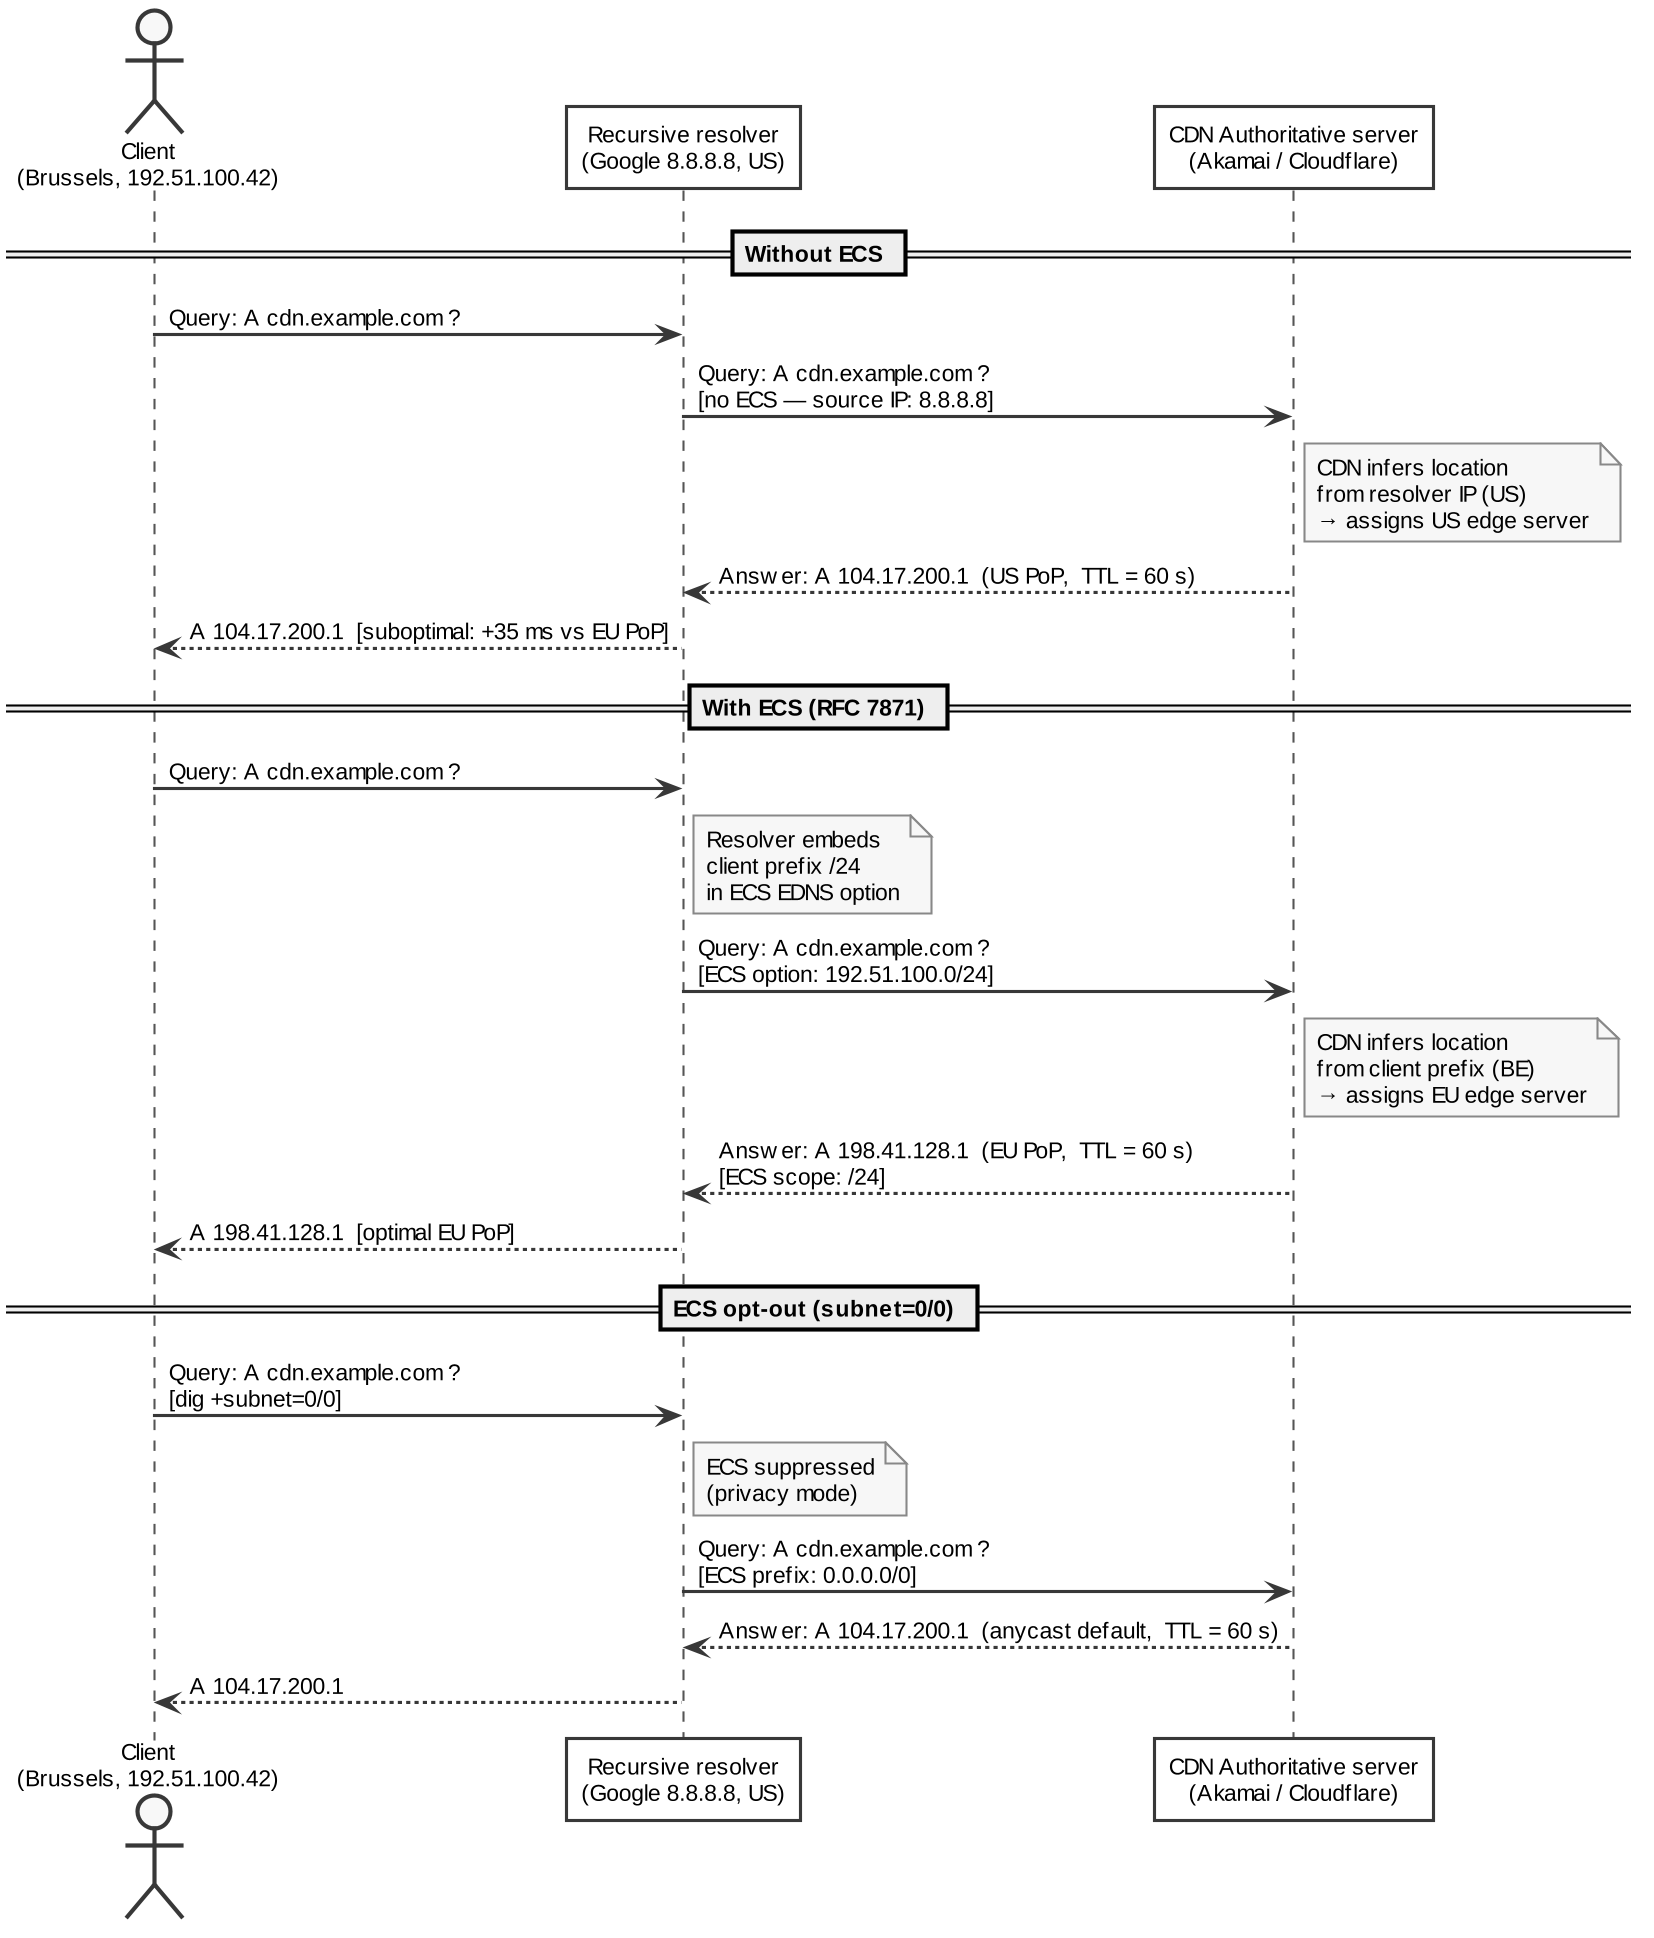
\includegraphics[width=0.90\linewidth]{figures/fig4_ecs_schema.png}
  \caption{Effect of \ac{ECS}~\cite{RFC7871} on \ac{CDN} geographic routing. \textit{Without \ac{ECS}}, the \ac{CDN} authoritative server infers client location from the recursive resolver's \ac{IP} (8.8.8.8, US), assigning a suboptimal US edge server to a Belgian client. \textit{With \ac{ECS}}, the resolver embeds the client's /24 prefix; the \ac{CDN} selects the geographically appropriate EU \ac{PoP}. \textit{\ac{ECS} opt-out} (\texttt{subnet=0/0}) suppresses the prefix entirely, reverting to resolver-\ac{IP}-based routing.}
  \label{fig:ecs_schema}
\end{figure}

\textbf{\ac{DNS} infrastructure centralisation}: Xu~\cite{Xu2023} show that over 90\% of forwarding resolvers are backed by fewer than 5\% of indirect recursive resolvers, and that just 10 \ac{DNS} providers serve 48.5\% of all g\ac{TLD} domain names. This centralisation creates a methodological choice between two complementary approaches, each with distinct trade-offs.

Using the probe's default resolver reflects the experience of real end-users: queries traverse the full recursive resolution chain, including the \ac{ISP} resolver's cache and any \ac{ECS} forwarding behaviour. This approach is appropriate for studying \ac{DNS} as users actually encounter it. Its limitation is that geographic diversity of probes may be partially unreal: two probes from different continents may share the same upstream recursive resolver, making their responses indistinguishable regardless of probe location.

Querying authoritative servers directly involves targeting the authoritative name server’s \ac{IP} and explicitly clearing the \ac{RD} bit, which effectively bypasses the recursive resolver layer. This approach ensures that each probe’s query hits the authoritative infrastructure from its own native \ac{IP} address, allowing us to cleanly isolate the geographic routing signal. A key trade-off, however, is that these metrics do not reflect the actual end-user experience mediated by the recursive resolver chain. The RIPE Atlas platform natively accommodates both of these operational approaches.

This thesis uses direct authoritative queries for Q1–Q3, where the goal is to characterise how the authoritative infrastructure responds to different geographic origins, and three major public resolvers (Cloudflare 1.1.1.1, Google 8.8.8.8, and Quad9 9.9.9.9) for Q4, where the goal is to compare resolver-induced differences in returned responses. The probe's local \ac{ISP} resolver was initially planned as a fourth condition but was abandoned: the RIPE Atlas API rejects the combination of an explicit target IP and \texttt{use\_probe\_resolver}: true, and probe inspection revealed that a large fraction of RIPE Atlas probes forward their local resolver to loopback addresses or directly to public resolvers, making the \ac{ISP} condition structurally indistinguishable from the public resolver conditions.

\section{Domain Ranking Lists}
\label{sec:2.6}

Studies of \ac{DNS} behaviour at scale require a reproducible domain corpus. Le Pochat~\cite{LePochat2019} evaluate four freely available ranking lists — Alexa, Cisco Umbrella, Majestic, and Quantcast — and find they agree on only 70,000 of a combined 2.82 million unique domains (24–33\% rank-biased overlap). Alexa’s 2018 methodology change caused 50\% daily list turnover, making longitudinal studies unreliable; Amazon subsequently shut down the Alexa ranking service entirely on 1 May 2022, making it unavailable for any ongoing research. Cisco Umbrella contains 51\% non-web entries (EC2 hostnames, typos). Majestic contains 2,162 documented malicious domains. All four lists are trivially manipulable: a single \ac{HTTP} request from an Alexa browser extension user can lift a domain to rank 28,798. Table~\ref{tab:ranking_lists} compares the main properties.

\begin{table}[tp]
\centering
\small
\begin{tabularx}{\linewidth}{p{2.2cm} X X X X}
\toprule
\textbf{Property} & \textbf{Alexa} \newline \textit{(discontinued 2022)} & \textbf{Cisco Umbrella} & \textbf{Majestic} & \textbf{Tranco} \\
\midrule
Data source  & Browser extension & \ac{DNS} queries to OpenDNS & Web crawl backlinks & Multi-source aggregation \\
Daily change rate & $\approx$50\,\% (post-2018) & $\approx$10\,\% & $\approx$1\,\% & $\approx$0.6\,\% \\
Manipulation effort & 1 \ac{HTTP} request & 1 \ac{DNS} query injection & Few backlinks & 4$\times$ vs single-source \\
Non-domain entries & Low & $\approx$51\,\% & Low & Filtered \\
Malicious domains & Some & Some & 2\,162 documented & Filtered \\
Reproducibility   & Daily overwrite & Daily overwrite & Daily overwrite & Stable permalink \\
\bottomrule
\end{tabularx}
\caption{Comparison of domain ranking lists. Tranco is the only list designed for research reproducibility and manipulation resistance~\cite{LePochat2019}.}
\label{tab:ranking_lists}
\end{table}

\textbf{Tranco}~\cite{LePochat2019} combines multiple ranking lists over a 30-day rolling window through the Borda count method. This aggregation yields a highly stable corpus with a minimal 0.6\% daily churn rate, while requiring a quadrupled adversarial effort across multiple lists to manipulate rankings. Furthermore, the framework ensures reproducibility by offering permanent, stable archived links. For the scope of this thesis, such stability guarantees that an identical set of domains is evaluated across all 128 daily campaigns, which is essential for conducting a robust temporal comparison.

\section{Synthesis and Research Positioning}
\label{sec:2.7}

The preceding review reveals a clear gap at the intersection of OpenINTEL’s temporal depth and RIPE Atlas’s spatial diversity. OpenINTEL provides daily, \ac{TLD}-wide \ac{DNS} measurement since 2015 but from a single Dutch vantage point: geographic variation is invisible. Existing RIPE Atlas \ac{DNS} studies are predominantly single-campaign, domain-limited case studies (a few hundred domains, one time point): Bortzmeyer~\cite{Bortzmeyer2013} studies a single anycast server; Finnegan~\cite{Finnegan2018} measures one resolver with 500 probes at a single instant; Hours~\cite{Hours2016} targets a handful of \ac{CDN} providers in one campaign; Koch~\cite{Koch2021} analyses root server anycast at one point in time. To date, no research has systematically quantified the exact fraction of popular domains returning geographically differentiated \ac{DNS} responses, nor have studies tracked the underlying driving mechanisms and their monthly evolution. Table~\ref{tab:gap_analysis} formalizes this academic positioning.

\begin{table}[tp]
\centering
\small
\begin{tabularx}{\linewidth}{p{2.8cm} p{3.5cm} p{3.8cm} X}
\toprule
\textbf{Dimension} & \textbf{OpenINTEL-based studies}~\cite{vanRijswijk2016} & \textbf{Existing RIPE Atlas studies}~\cite{Bortzmeyer2013,Finnegan2018,Hours2016,Koch2021} & \textbf{This thesis} \\
\midrule
Domain coverage  & Full \ac{TLD} zone files & Experimenter-defined (per study) & Tranco Top-250 (stable, reproducible) \\
Geographic vantage    & Single point (Netherlands) & $\approx$12\,900 probes, 178 countries & Multi-continent stratification \\
Temporal depth & Daily since March 2015 & Single campaigns & 127-day repeated campaigns \\
Anycast tracking       & Not applicable & Case studies (d.nic.fr, UncensoredDNS) & Systematic across corpus \\
Resolver control   & Fixed central resolver & Local probe resolver (default) & Direct authoritative query \\
\bottomrule
\end{tabularx}
\caption{Positioning of this thesis relative to existing \ac{DNS} measurement infrastructure across five dimensions.
All three columns represent measurement studies; Each row identifies a gap that this work explicitly addresses.}
\label{tab:gap_analysis}
\end{table}

Three critical gaps in the existing literature form the core motivation for this thesis:

\begin{itemize}
\item \textbf{Limitation 1: Absence of population-scale \ac{DNS} characterization}. Prior literature consists largely of isolated anycast case studies (\cite{Bortzmeyer2013,Finnegan2018}) and targeted \ac{CDN} routing analyses (\cite{Hours2016,Li2025}) that focus on a single service or domain at a time. Consequently, the research landscape lacks a comprehensive measurement showing what percentage of the popular-domain ecosystem exhibits geographic differentiation, as well as which mechanisms dominate at scale.

\item \textbf{Limitation 2: Resolver centralization obscuring vantage-point diversity}. Relying on local probe resolvers often introduces an artificial layer of geographic diversity that ultimately vanishes at the resolution layer. This occurs because nearly 90\% of forwarding resolvers consolidate into a mere 5\% of recursive resolvers\cite{Xu2023}. While direct authoritative querying serves as the necessary remedy to bypass this bottleneck, none of the current case studies explicitly document this approach as a core architectural design choice.

\item \textbf{Limitation 3: Lack of temporal dynamics in snapshot studies}. As acknowledged by Koch~\cite{Koch2021} and Bortzmeyer ~\cite{Bortzmeyer2013}, \ac{BGP} routing policies and \ac{CDN} anycast catchments are inherently volatile, changing continuously as operators deploy new \ac{PoPs} or restructure peering agreements. Capturing the true stability of geographic \ac{DNS} response differentiation therefore requires a long campaign rather than a single-snapshot measurement.
\end{itemize}

This thesis addresses all three gaps by deploying a measurement system that queries the Tranco Top-250 directly at authoritative servers from $\approx$200 geographically stratified RIPE Atlas probes, repeated daily over 127 days, with \ac{NSID}-based anycast instance tracking and results archived in Parquet following \ac{FAIR} data principles.